\documentclass[paper=a4, fontsize=11pt]{scrartcl}
\usepackage[T1]{fontenc}
\usepackage{fourier}

\usepackage[english]{babel}															% English language/hyphenation
\usepackage[protrusion=true,expansion=true]{microtype}	
\usepackage{amsmath,amsfonts,amsthm} % Math packages
\usepackage[pdftex]{graphicx}	
\usepackage{url}
\usepackage{hyperref}


%%% Custom sectioning
\usepackage{sectsty}
\allsectionsfont{\centering \normalfont\scshape}
\usepackage{subfigure}
\usepackage{comment}


%%% Custom headers/footers (fancyhdr package)
\usepackage{fancyhdr}
\pagestyle{fancyplain}
\fancyhead{}											% No page header
\fancyfoot[L]{}											% Empty 
\fancyfoot[C]{}											% Empty
\fancyfoot[R]{\thepage}									% Pagenumbering
\renewcommand{\headrulewidth}{0pt}			% Remove header underlines
\renewcommand{\footrulewidth}{0pt}				% Remove footer underlines
\setlength{\headheight}{13.6pt}


%%% Equation and float numbering
%\numberwithin{equation}{section}		% Equationnumbering: section.eq#
%\numberwithin{figure}{section}			% Figurenumbering: section.fig#
%\numberwithin{table}{section}				% Tablenumbering: section.tab#


%%% Maketitle metadata
\newcommand{\horrule}[1]{\rule{\linewidth}{#1}} 	% Horizontal rule

\title{
		%\vspace{-1in} 	
		\usefont{OT1}{bch}{b}{n}
		\normalfont \normalsize \textsc{CS650 - Computer Vision} \\ [25pt]
		\horrule{0.5pt} \\[0.4cm]
		\huge Programming Lab 4 \\ Pattern Recognition Basics \\
		\horrule{2pt} \\[0.5cm]
}
\author{
		\normalfont 								\normalsize
        Daqing Yi\\[-3pt]		\normalsize
        \today
}
\date{}


%%% Begin document
\begin{document}
\maketitle

\begin{comment}
prepare a brief writeup to submit.
Your writeup should document your features and your algorithms as well as describe any observations you have made and ideas you have for how to improve the results.
Don't forget to document your code.

Descriptor
compactness, rectangularity, eccentricity, moments, elongation, psi-s curves, profiles, holes, corners, etc.
\end{comment}

\section{Introduction}
\label{sec:intro}

This lab implements a basic pattern recognition on the objects in binary images.
The implementations are written in Python.
CV2 (open CV) is used for reading image files into data arrays.
Numpy is used for array operations.
Matplotlib is used for visualizing data.

In this lab, the objects are firstly extracted from the image.
The features of the object are quantized into points in feature space.
A minimum distance classifier is used to separate the objects into five classes by shape features.
The results are also tested on other image files to verify generalization capability.

\section{Object isolation}
\label{sec:object_isolation}

The test image files are firstly loaded into binary image.
The binary image is maintained by a \textbf{PixelGraph} class in \emph{PixelGraph.py}.
Connected-Component labeling \footnote{\url{http://en.wikipedia.org/wiki/Connected-component_labeling}}
is used to isolate the objects from binary image.
Each 
The implementation follows the ``two-pass algorithm'' described in \cite{wiki:connected_component_labeling}.
A \textbf{ConnectedComponentMgr} in \emph{ConnectedComponent.py} is used to maintain the connected components found.
The ``two-pass'' process is implemented in \emph{\_\_init\_\_(self, data)}.
The first pass assigns a label to each pixel, and adds neighbored labels into union set.
The second pass merges the labels in same union set into one label.
I add an extra pass to make the unique label sequential. 
Each component is assigned an index as ID by sequence.
Seome examples are given in Figure \ref{fig:obj_iso}.

\begin{figure}[h]
\centering
\subfigure[Object Index 2 of \emph{shapes.pgm}]{
\includegraphics[width=.3\textwidth]{./figure/shapes_obj2} 
\label{fig:obj_iso:01} } 
\subfigure[Object Index 3 of \emph{train1.pgm}]{
\includegraphics[width=.3\textwidth]{./figure/train1_obj3} 
\label{fig:obj_iso:02} } 
\subfigure[Object Index 4 of \emph{match1.pgm}]{
\includegraphics[width=.3\textwidth]{./figure/match1_obj4} 
\label{fig:obj_iso:03} } 
\caption{Object isolation.}
\label{fig:obj_iso}
\end{figure}

\begin{figure}[h]
\centering
\subfigure[Object Index 2 of \emph{shapes.pgm}]{
\includegraphics[width=.3\textwidth]{./figure/shapes_cc2} 
\label{fig:obj_cc:01} } 
\subfigure[Object Index 3 of \emph{train1.pgm}]{
\includegraphics[width=.3\textwidth]{./figure/train1_cc3} 
\label{fig:obj_cc:02} } 
\subfigure[Object Index 4 of \emph{match1.pgm}]{
\includegraphics[width=.3\textwidth]{./figure/match1_cc4} 
\label{fig:obj_cc:03} } 
\caption{Contour finding.}
\label{fig:obj_cc}
\end{figure}

\section{Feature extraction}
\label{sec:feature_extraction}

A \emph{ShapeDescriptor} class in \emph{ShapeDescriptor.py} is used to generate shape features of a connected component.
In this label, the extracted features are listed as following.

\begin{itemize}
\item \textbf{Compactness} 

Compactness indicates how compact a shape is, which is measured by $ \mbox{perimeter}^{2} / \mbox{area} $.
$ \mbox{area} $ is counted by the pixel number.
$ \mbox{perimeter} $ is calculated from the contour. 
The contour is in the form of the chain code \footnote{\url{http://en.wikipedia.org/wiki/Chain_code}}. 
The algorithm is implemented following \cite{chaincode}.
The contours found can be used to calculate the perimeter of the object.
Figure \ref{fig:obj_cc} shows how the contours of the objects are like.,

\item \textbf{Rectangularity} 

Rectanglarity indicates how close a shape to a rectangle.
It is defined by the ration of the area of the object and the area of its minimum bounding rectangle.

\begin{figure}[h]
\centering
\subfigure[Convex hull]{
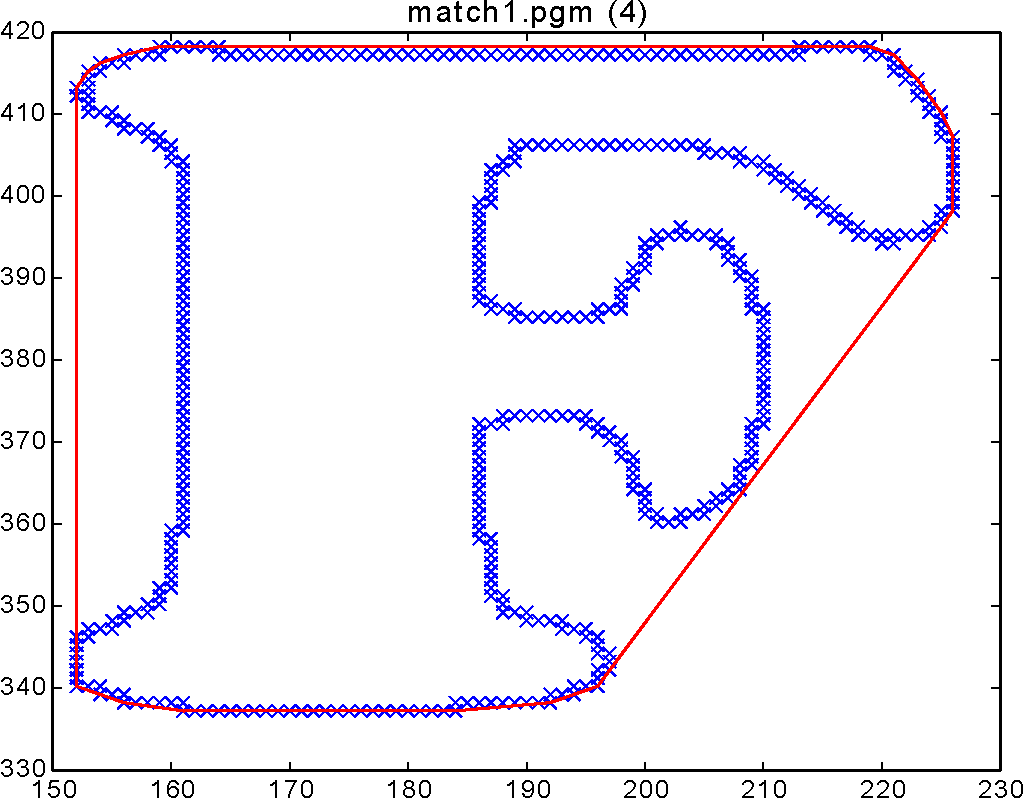
\includegraphics[width=.3\textwidth]{./figure/match1_convex_hull_4} 
\label{fig:convex_hull} } 
\subfigure[Minimum bounding rectangle]{
\includegraphics[width=.3\textwidth]{./figure/match1_min_rect_4} 
\label{fig:min_bound_box} } 
\caption{Convex hull and minimum bounding rectangle.}
\label{fig:convex_hull_min_bound_box}
\end{figure}

The minimum bounding rectangle is generated by rotating a rectangle to find an angle that minimize the bounding area.
The implementation is in \textbf{ getMinimumBoundingBox(points) } in \emph{boundingShape.py}.

\item \textbf{Eccentricity}

Eccentricity is also obtained from a minimum bounding rectangle.
It is calculated by the ratio of its width and height.
A square object or a circle object should have eccentricity equals to one.
It can be used to differentiate a rectangle with a square and an ellipse with a circle.

\item \textbf{Elongation}

Elongation is defined as $ 1 - \mbox{eccentricity} $.
It measures the eccentricity in an opposite direction.

\item \textbf{Hole area ratio}

Hole area ratio is used to evaluate the hole area inside an object.
It is measured by the ratio of the object area and its contour area.
The hole area ratio of the object in Figure \ref{fig:obj_iso:01} is $ 0.6567 $.
While the hole area ratio of the object in Figure \ref{fig:obj_iso:03} is $ 0.9439 ( \approx 1 ) $.

\item \textbf{Solidity}

Solidity indicates how an object approximates its convex hull.
It is measured by the ratio of the contour area and the area of the convex hull.
If an object is a rectangle, solidity is closed to 1.

\item \textbf{Convexity}

The convexity is another way to indicates an object approximates its convex hull.
It is measured by the ratio of the perimeter of the contour and the perimeter of the convex hull.

\item \textbf{Ellipse ratio}

Ellipse ratio measures how an object approximates an ellipse.
From a minimum bounding rectangle, an ellipse can be obtained by its width and height.
Ellipse ratio is calculated by the ratio of the ellipse area and the contour area. 

\item \textbf{Moments}

In order to ignore the difference from rotation, Hu invariant set is used to evaluate the moments features.
Let
\begin{equation}
m_{ij} = \sum ( x - \bar{x} )^{i} ( y - \bar{y} )^{j},
\end{equation}
the Hu invariant set is defined as 
\begin{subequations}
\begin{equation}
M_{1} = m_{20} + m_{02}
\end{equation}
\begin{equation}
M_{2} = (m_{20} + m_{02})^{2} + 4 m_{11}^{2}
\end{equation}
\begin{equation}
M_{3} = (m_{30} - 3m_{12})^{2} + (3m_{21}-m_{03})^{2}
\end{equation}
\begin{equation}
M_{4} = (m_{30} + m_{12})^{2} + (m_{21} + m_{03})^{2}
\end{equation}
\begin{equation}
\begin{aligned}
M_{5} = & (m_{30} - 3m_{12})( m_{30}+ m_{12} ) [ (m_{30} + m_{12})^{2} - 3(m_{21} + m_{03})^{2} ] \\
 & + (3 m_{21}- m_{03})(m_{21} + m_{03})[ 3(m_{30} + m_{12})^{2}-(m_{21} + m_{03})^{2} ]
 \end{aligned}
\end{equation}
\begin{equation}
\begin{aligned}
M_{6} = & (m_{20}+m_{02}) [ (m_{30} + m_[12])^{2} - 3 (m_{21} + m_{03})^{2} ] \\
 & + 4 m_{11} (m_{30} + m_{12}) ( m_{03} + m_{21} )
\end{aligned} 
\end{equation}
\begin{equation}
\begin{aligned}
M_{7} = & (3 m_{21} - m_{03}) ( m_{12} + m_{30}) [ m_{30} + m_{12}^{2} - 3(m_{21} + m_{03} )^{2} ] \\ 
& - (m_{30} - 3 m_{12}) (m_{12} + m_{03}) [ 3 ( m_{30} + m_{12} )^{2} - (m_{21} + m_{03})^{2} ]
\end{aligned}
\end{equation}
\end{subequations}

These seven values are set into the feature vector for classification.

\end{itemize}

All the feature values are normalized into $ [0, 1] $.
It enables the weights of different features can be manually tuned later.

\begin{figure}[h]
\centering
\includegraphics[width=0.7\linewidth]{./figure/kmean}
\caption{Minimum Distance classifier.}
\label{fig:min_dist_classifer}
\end{figure}

\section{Minimum distance classifier}
\label{sec:classifier}

A minimum distance classifier is used to classify the objects by features.
Because a 5 separate pattern clustering is required.
K-means clustering is firstly used to find the mean of each cluster.
The means are then used by a minimum-distance classifier.
In this multiple classes case, there is a single linear discriminant $ g_{i} ( \mathbf{x} ) $ for each class $ \omega_{i} $.
The class $ \omega_{i} $ is assigned to $ \mathbf{x} $ if $ \forall j \neq i, g_{i} ( \mathbf{x} ) > g_{j} ( \mathbf{x} ) $.
$ g_{i}( \mathbf{x} ) $ is defined as 
\begin{equation}
g_{i}( \mathbf{x} ) = \mathbf{x}^{T} \mathbf{m}_{i} - \frac{1}{2} \mathbf{m}_{i}^{T} \mathbf{m}_{i}.
\end{equation}
Because minimizing $ || \mathbf{x} - \mathbf{m}_{i} || $ is equivalent to maximizing $ \mathbf{x}^{T} \mathbf{m}_{i} - \frac{1}{2} \mathbf{m}_{i}^{T} \mathbf{m}_{i} $.
Figure \ref{fig:min_dist_classifer} gives an example of the minimum distance classifier.
A set of 2D positions are randomly generated.
The k-means firstly finds the means of five clusters.
A minimum-distance classifier can then classify the positions into five labels, which are visualized in different colors in Figure \ref{fig:min_dist_classifer}.


\section{Pattern recognition}
\label{sec:pattern_recognition}

\begin{figure}[h]
\centering
\subfigure[Training]{
\includegraphics[width=.45\textwidth]{./figure/shapes_pgm-0} 
\label{fig:class:01:train} } 
\subfigure[Testing]{
\includegraphics[width=.45\textwidth]{./figure/testshapes_pgm-0} 
\label{fig:class:01:test} } 
\caption{Classifications on \emph{shapes.pgm} and \emph{testshapes.pgm}.}
\label{fig:class:01}
\end{figure}

Given different types of objects to classify, different types of features might have different importance.
Particularly when some feature does not help the classification, its weight can be set to zero. 

Features are firstly extracted from the objects in \emph{shapes.pgm}.
The feature vectors are then used to train a minimum-distance classifier.
Later the features of the objects in \emph{testshapes.pgm} are extracted and sent to the minimum-distance classifier for labeling.
Figure \ref{fig:class:01} gives the labeling results on \emph{shapes.pgm} and \emph{testshapes.pgm} by colors.
\textbf{Compactness} and \textbf{Rectangularity} can be enough to classify the objects into five classes.
\emph{classify01.py} is the test file to verify the result of the train file \emph{shapes.pgm}.
\emph{classify02.py} is the test file to show the results of both the train file \emph{shapes.pgm} and the test file \emph{testshapes.pgm}.
If more features are enabled, the classification result can still be correct by weighing them reasonably.

\begin{figure}
\centering
\subfigure[Training 1]{
\includegraphics[width=.45\textwidth]{./figure/train1_pgm-0} 
\label{fig:class:02:train1} } 
\subfigure[Training 2]{
\includegraphics[width=.45\textwidth]{./figure/train2_pgm-0} 
\label{fig:class:02:train2} }
\\
\subfigure[Testing 1]{
\includegraphics[width=.45\textwidth]{./figure/match1_pgm-0} 
\label{fig:class:02:match1} } 
\subfigure[Testing 2]{
\includegraphics[width=.45\textwidth]{./figure/match2_pgm-0} 
\label{fig:class:02:match2} }
\caption{Classifications on \emph{train1.pgm}, \emph{train2.pgm}, \emph{match1.pgm} and \emph{match2.pgm}.}
\label{fig:class:02}
\end{figure}

Similarly, the objects in \emph{train1.pgm} and \emph{train2.pgm} are used to train a minimum-distance classifier.
The objects in \emph{match1.pgm} and \emph{match2.pgm} are used to test.
But more features are enabled in this case.
Figure \ref{fig:class:02} gives the labeling results on \emph{train1.pgm}, \emph{train2.pgm} and \emph{match1.pgm} \emph{match2.pgm} by colors.
\emph{classify03.py} is the test file to verify the result of the train files \emph{train1.pgm} and \emph{train2.pgm}.
\emph{classify04.py} is the test file to show the results of both the train files \emph{train1.pgm} and \emph{train2.pgm} and the test files \emph{match1.pgm} and \emph{match2.pgm}.
Most of the objects can be correctly labeled. 
The difficulty is in distinguishing ``E'' and ``F''.
Tuning the weights of some features, like hole area ratio, can change the classification result of the ``E'' objects and the ``F'' objects. 
But there is still some mislabeling.
A feature that can distinguish ``E'' with ``F'' significantly is needed here.

\section{Summary}

The features chosen for classification determines the criterion of object classification.
For instance, a square object can be labeled into the same class with a circle object if only \textbf{rectangularity} is used.
It can also be labeled into the same class with a rectangle object if only \textbf{compactness} is used.

When the features are enough to classify the objects, importing new feature might bring mislabeling.
Because all the features are normalized, assigning correct weights to the features is also very important to generate the expected labeling results.


\bibliography{reference}
\bibliographystyle{plain}

\end{document}